\documentclass[12pt]{article}

\usepackage[italian]{babel}
\usepackage{graphicx} 
\usepackage{etaremune}
\usepackage{fancyhdr}
\usepackage[a4paper,top=2.8cm,bottom=2.8cm,left=2.4cm,right=2.4cm]{geometry}
%\usepackage[export]{adjustbox}
%\usepackage{wrapfig}
\usepackage{subcaption}
\usepackage{float}
\usepackage{listings}

\lstset{basicstyle=\ttfamily,
  showstringspaces=false,
  basicstyle=\footnotesize\ttfamily,
  numbers=left,
  stepnumber=1,
  numbersep=10pt,    
  columns=fullflexible,
  frame=single,
  breaklines=true,
  numberstyle=\small
}

\title{Relazioni Internet}
\author{Squadra A\\Gruppo 16}
\date{}

\lhead{
\begin{minipage}[c][2cm][c]{\textwidth}
 \textbf{Laboratori di internet e comunicazioni}
\end{minipage}
}
\rhead{
\includegraphics[width = 2.5cm]{logo_poli.png}}
\renewcommand{\headrulewidth}{0pt}
\setlength{\headheight}{3cm}

\pagestyle{plain}

\begin{document}


\maketitle	
\thispagestyle{fancy}


\newpage

\setcounter{page}{1}
\setlength{\headheight}{0cm}

\section{Quarto laboratorio}
In questo laboratorio si abbiamo utilizzato il client e server \textbf{nttcp} per seguire dei test relativi alla velocità di trasmissione tra più host in diversi scenari.\\
In particolare sono stati utilizzati 3 host, che chiameremo H1 ,H2 e H3, ognuno dei quali utilizzava una scheda di rete Intel. Ciascun host è stato collegato a uno switch attraverso un cavo ethernet e la sua scheda di rete è stata configurata in maniera diversa in base allo scenario desiderato.
Nella configurazione di quest'ultima si è intervenuti su velocità e tipo di connessione (half o full duplex).
Per fare ciò abbiamo utilizzato \textbf{ethtool} e la seguente sintassi.
\begin{verbatim}
sudo ethtool -s eth0 speed [velocità] duplex [full|half] autoneg on
\end{verbatim}
H1 e H2 sono stati settati per comunicare alla velocità di 10 Mb/s, mentre H3 a 100 Mb/s. Tutti gli host sono stati configurati in full duplex.\\
Inseguito sono state disabilitate le funzioni avanzate della scheda di rete per evitare la segmentazione (\textit{vedi sezione 2}) aggiungendo il seguente comando per disattivare il  protocollo \textbf{PAUSE frame}, che permetterebbe allo switch di evitare congestioni (cosa che noi vogliamo accada), con il seguente comando.
\begin{verbatim}
sudo ethtool -T eth0 autoneg off rx off tx off
\end{verbatim}	
Inoltre per identificare la trasmissione di dati tra 2 host sono state usate delle sigle, in particolare:
\renewcommand{\theenumi}{F\arabic{enumi}}
\begin{enumerate}
\item H1 invia dati a H3
\item H3 invia dati a H2
\item H1 invia dati a H2
\end{enumerate}
Nel corso dei vari test abbiamo catturato i pacchetti scambiati con \textbf{wireshark} e generato i grafici della velocità utilizzando la funzione \textbf{grafici I/O}.

\subsection{TCP}
In questo primo scenario abbiamo utilizzato nttcp senza specificare opzioni, utilizzando \textbf{nttcp -T}.
Così facendo il client invierà 2048 pacchetti lunghi 4096 utilizzando TCP.\\
Sono state aperte 3 connessioni: F1, F2 ed F3.
Ciò che ci aspettiamo è che le due connessioni F1 ed F3 si dividano equamente la banda (5 Mb/s a testa), tuttavia non è ciò che accade.\\
Come possiamo notare dal grafico in \textit{figura 1}, F1 sarà più veloce. Ripetendo più volte il test notiamo che tale situazione si ripete e che dunque non è un caso che F1 sia più veloce di F3. 
Possiamo ipotizzare che F3 sarà più lento in quanto si ritoverà costretto a dover utilizzare solo segmenti di cavo ethernet che dovrà condividere con altre connessioni, mentre nel caso di F2 ed F1 solo una delle due sezioni attraversate dovrà essere condivisa. Dunque nel tratto che collega lo switch ad H2 vi sarà una congestione che porterà F3 a perdere dei pacchetti, mentre sul tratto che collega lo switch ad H3 non ci sarà congestione e F1 e F2 saranno soggetti a una minore perdita di pacchetti e di conseguenza potranno andare più veloci.
Notare inoltre che tra i 2.8 e i 10.2 secondi vi è stato un crollo e una risalita della velocità di F3 e F1. Ciò è dovuto alla congestione tra i 2 nel tratto di cavo da loro condiviso. Entrambi aumenteranno la loro finestra per aumentare la velocità e una volta raggiunti valori troppo alti il controllo di TCP li porterà a rallentare.

\begin{figure}[H]
	\noindent\makebox[\textwidth]{%
	\begin{subfigure}[l]{0.5\textwidth}
		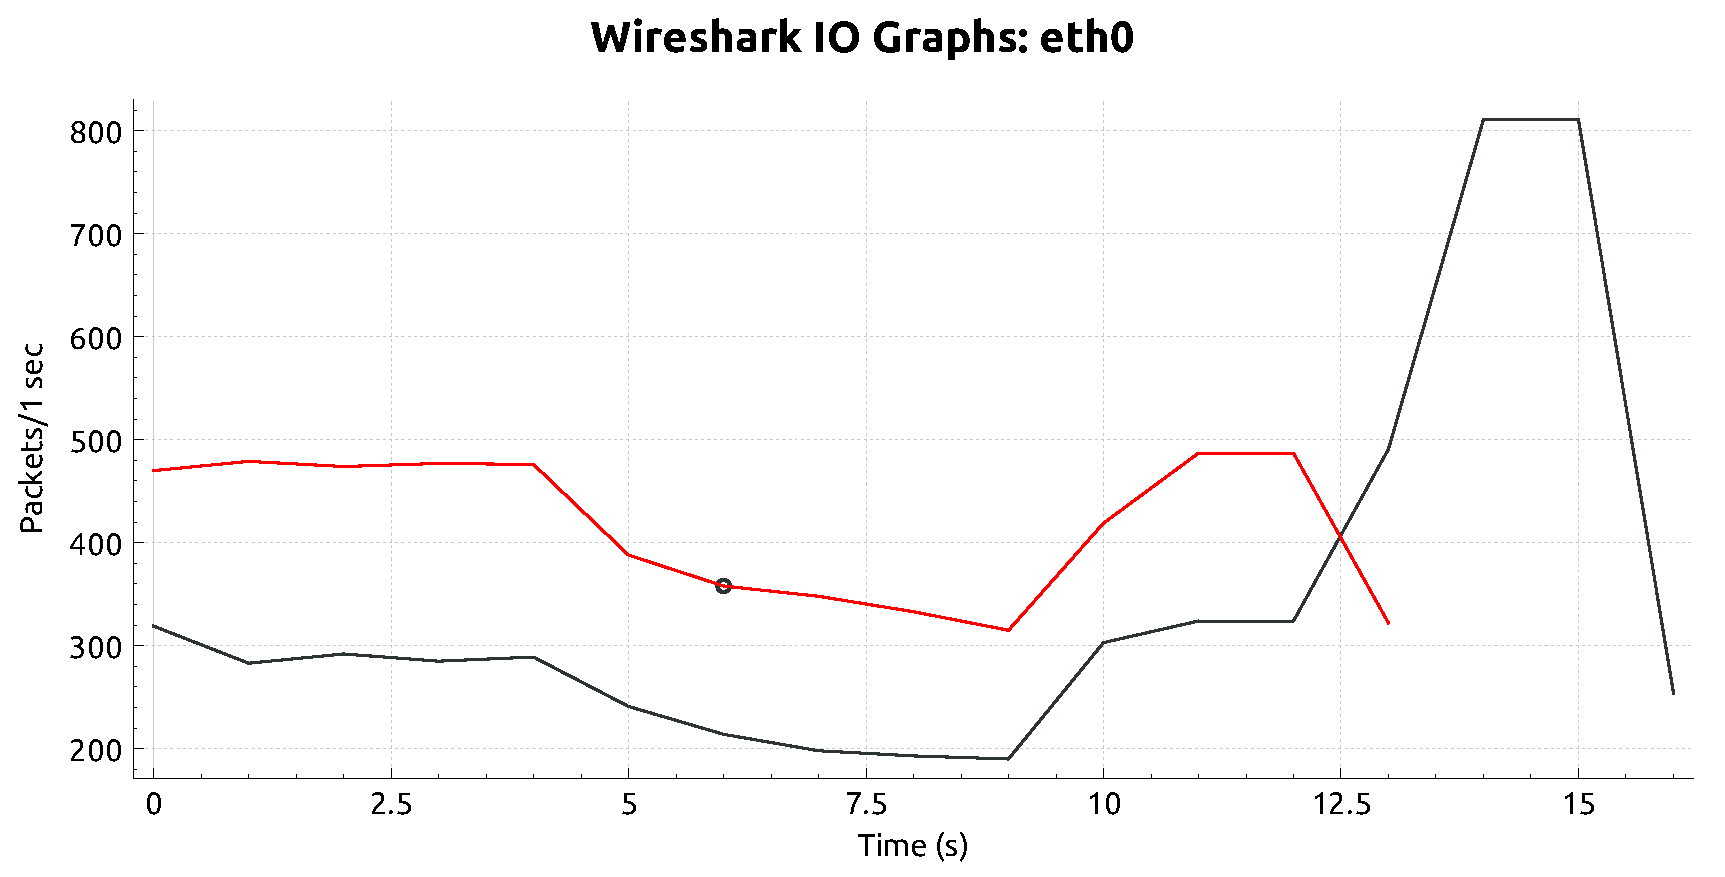
\includegraphics[width=\linewidth]{TCP_H1_test1.pdf}
		\caption{Velocità F3(nero) e F1(rosso) viste da H1}
	\end{subfigure}	
	\begin{subfigure}[r]{0.6\textwidth}
		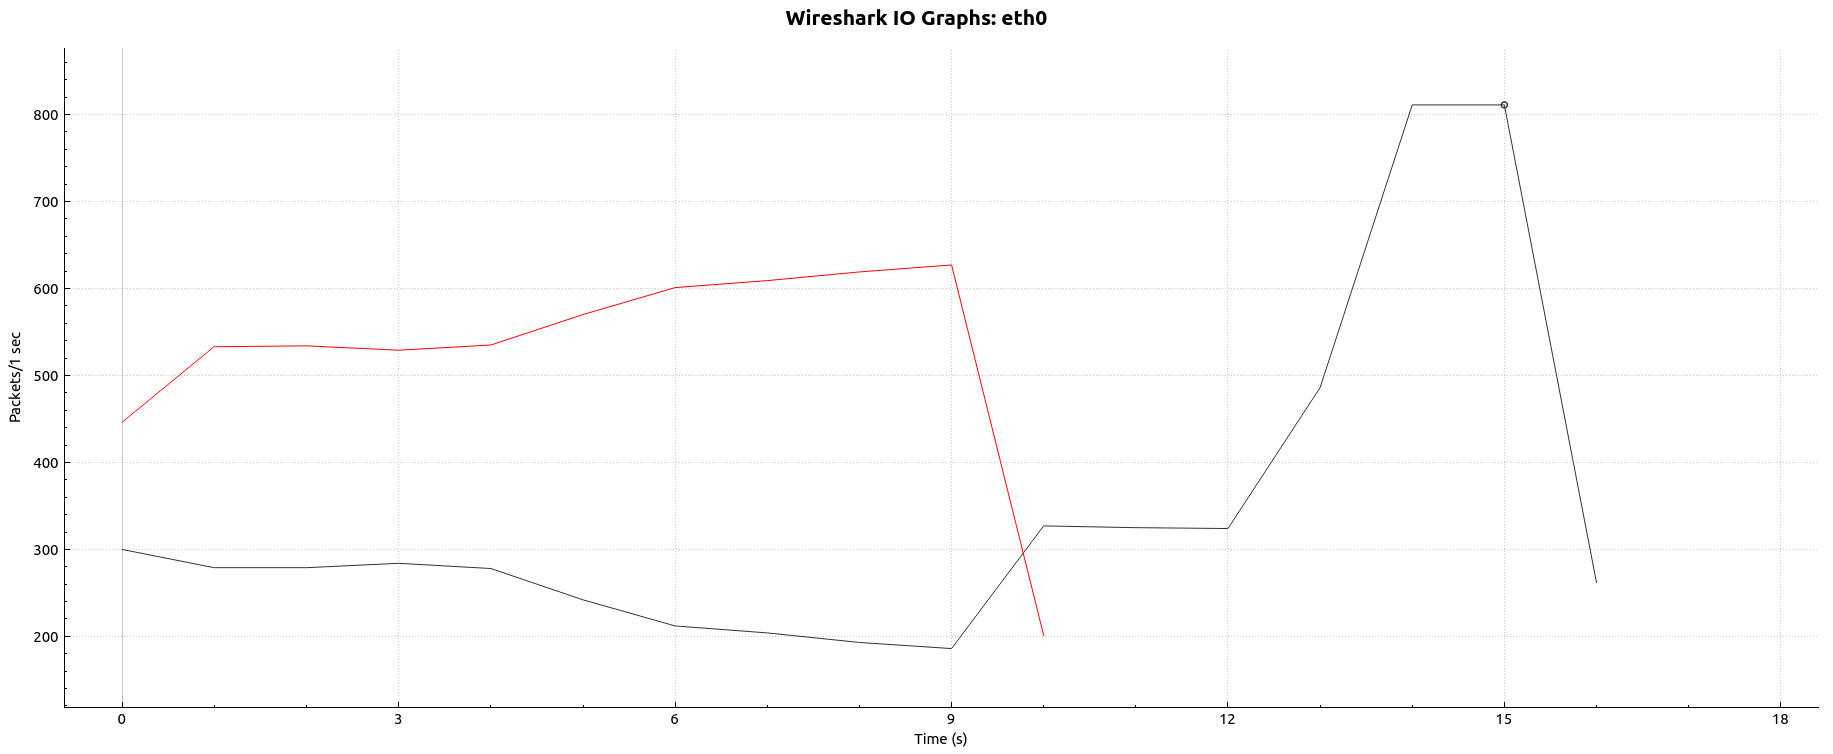
\includegraphics[width=\linewidth]{TCP_H2_test1.png}
		\caption{Velocità F3(nero) e F2(rosso) viste da H2}
	\end{subfigure}}
	\caption{Diagrammi velocità in TCP}
\end{figure}

\subsection{UDP}
In questo secondo scenario abbiamo utilizzato nttcp sfruttando UDP.
E' stato utilizzato il seguente comando: \textbf{nttcp -T -u -l 1472}.
Notare l'opzione -l che impone una lunghezza dei pacchetti inviati di 1472 in modo da inviare pacchetti UDP di dimensione massima senza ricadere nella frammentazione che avverrebbe a livello ip per pacchetti più grossi.
Come in precedenza sono state aperte 3 connessioni: F1, F2 ed F3.
Ciò che ci aspettiamo è uno scenario in cui, non essendoci controlli di congestione, ogni canale verrà sfruttato al massimo della propria velocità.
Sono stati fatti diversi test.

\subsubsection{Test 1}
Ciò che notiamo nel grafico in \textit{figura 3} è un' equa divisione della velocità della banda tra F1 e F3 in quanto i loro pacchetti verranno inviati dallo stesso host. 
Infatti il segmento a 100 mb/s attraversato da F1 non inciderà sulla sua velocità di trasmissione in quanto essa dipenderà unicamente dalla scheda di rete del client. Ciò che avviene è che i buffer dello switch verranno "riempiti" a una velocità inferiore rispetto a quella con cui potranno "scaricarsi". Il che si traduce con l'assenza di congestioni dovute a F1 e F3, come si evince dai seguenti output di nttcp, i quali non mostrano perdite di pacchetti.
\begin{verbatim}
F3
  Bytes  Real s   CPU s Real-MBit/s  CPU-MBit/s   Calls  Real-C/s   CPU-C/s
3014656    4.87    0.01      4.9542   2961.7153    2051    421.32  251872.8
3014656    5.02    0.06      4.8036    391.8191    2049    408.12   33288.9

F1
  Bytes  Real s   CPU s Real-MBit/s  CPU-MBit/s   Calls  Real-C/s   CPU-C/s
3014656    4.92    0.01      4.8974   2902.8946    2051    416.49  246870.5
3014656    4.93    0.10      4.8888    237.9201    2049    415.35   20213.7
\end{verbatim}
Per quanto riguarda F2 possiamo notare dal grafico in \textit{figura 4} che la mancanza di controlli di congestione unita a un' elevata velocità di trasferimento, causerà congestione e perdita di pacchetti.
\begin{verbatim}
FILE MANCANTE.... TROVARE SOLUZIONE
\end{verbatim}
Ciò avviene in quanto i buffer dello switch verranno "riempiti" molto più velocemente di quanto possano essere "svuotati" e  dunque, non avendo più spazio, sarà costretto a scartare i pacchetti in entrata.
Notare inoltre che F2 riesce a saturare la banda in modo da impedire la trasmissione di F2 e F3, che inizieranno a comunicare in ritardo. Questo perchè nttcp prima di iniziare a comunicare  crea una connessione tra client e server usando protocollo TCP, indipendentemente dal protocollo utilizzato per il test. Dunque F3 impedirà lo scambio di SYN e ACK necessarie alla connessione, che verranno perse a causa della congestione.\\
Notare inoltre che la massima velocità di F2 sarà di soli 81 Mb/s a differenza dei 96 Mb/s previsti dalla teoria.
Ciò accade a causa della scheda di rete Intel che limita la velocità di UDP.

\begin{figure}[H]
	\noindent\makebox[\textwidth]{%
	\begin{subfigure}[l]{0.5\textwidth}
		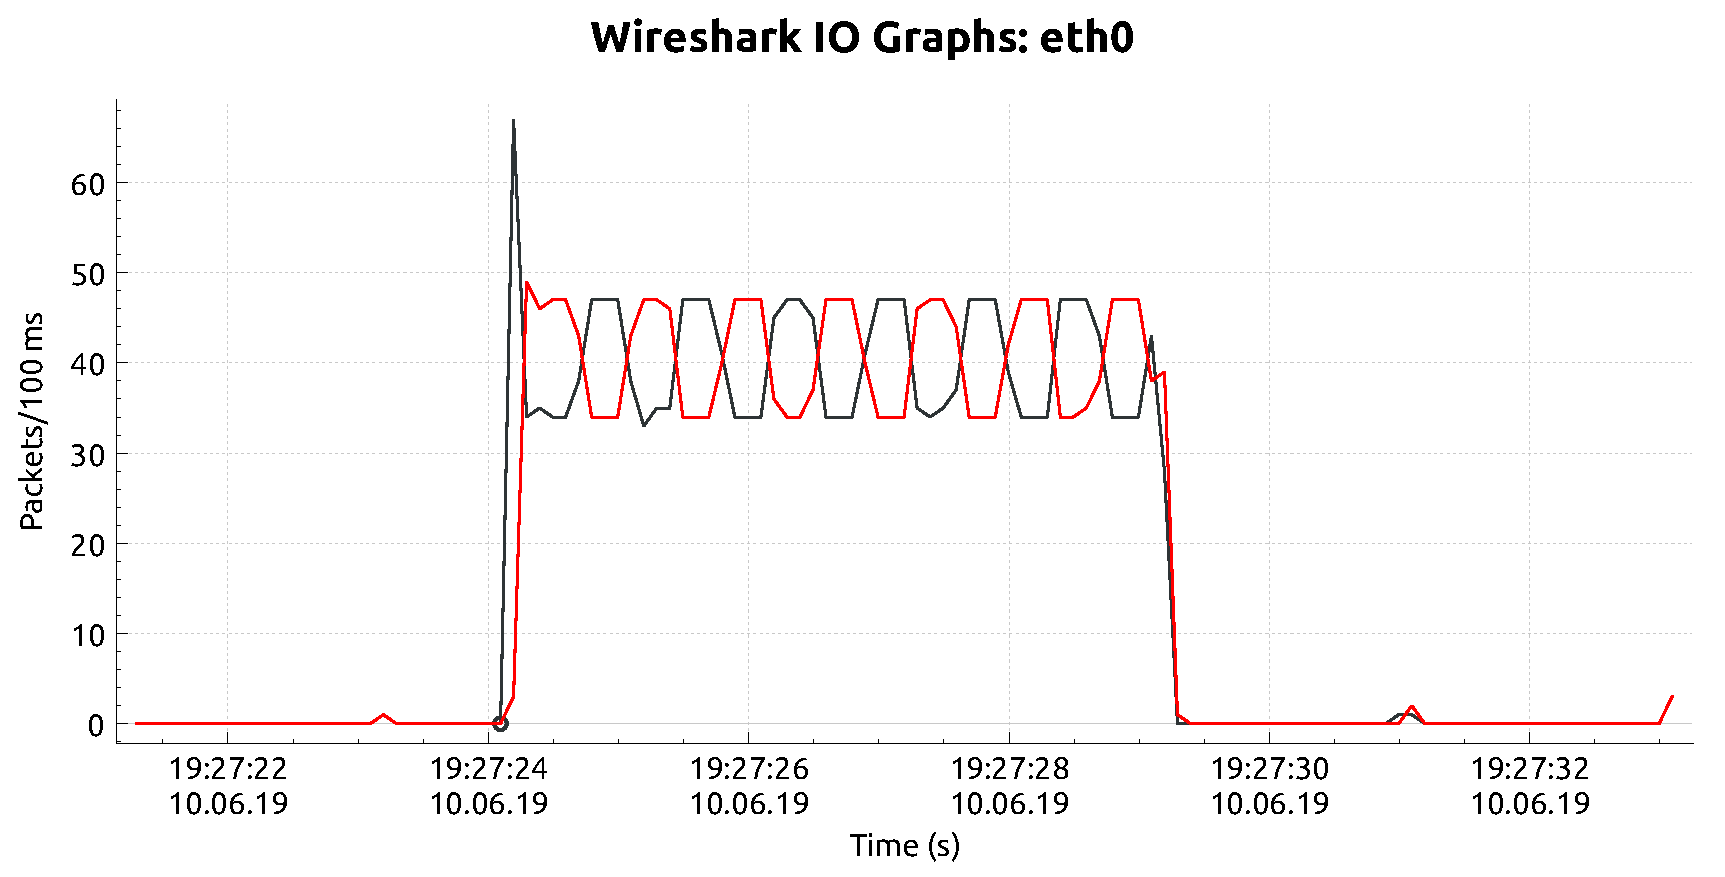
\includegraphics[width=\linewidth]{UDP_H1_test1.pdf}
  		\caption{Velocità F3(nero) e F1(rosso) viste da H1}
	\end{subfigure}	
	\begin{subfigure}[r]{0.5\textwidth}
		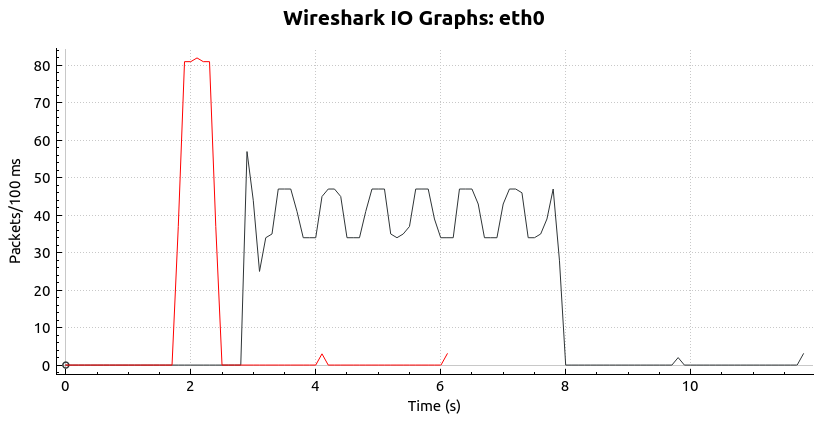
\includegraphics[width=\linewidth]{UDP_H2_test1.png}
  		\caption{Velocità F3(nero) e F2(rosso) viste da H2}
	\end{subfigure}}
	\caption{Diagrammi velocità in UDP (test 1)}
\end{figure}

\subsubsection{Test 2}
In questo test abbiamo aumentato il numero di pacchetti utilizzati da F2, in modo da impedire a quest'ultima di terminare prima dell'inizio di F1 e F3.
Ciò che abbiamo osservato nei grafici in \textit{figura 5} e \textit{figura 6} è appunto una F2 più duratura, ma che tuttavia impedirà, come nel caso precedente, la connessione di F3 e F1 con un effetto tuttavia diverso. Se prima F2 terminava abbastanza velocemente, ora impiegherà così tanto tempo da causare il timeout di F3 e F1, che non riusciranno di conseguenza a connettersi.

\begin{figure}[H]
	\noindent\makebox[\textwidth]{%
	\begin{subfigure}[l]{0.51\textwidth}
		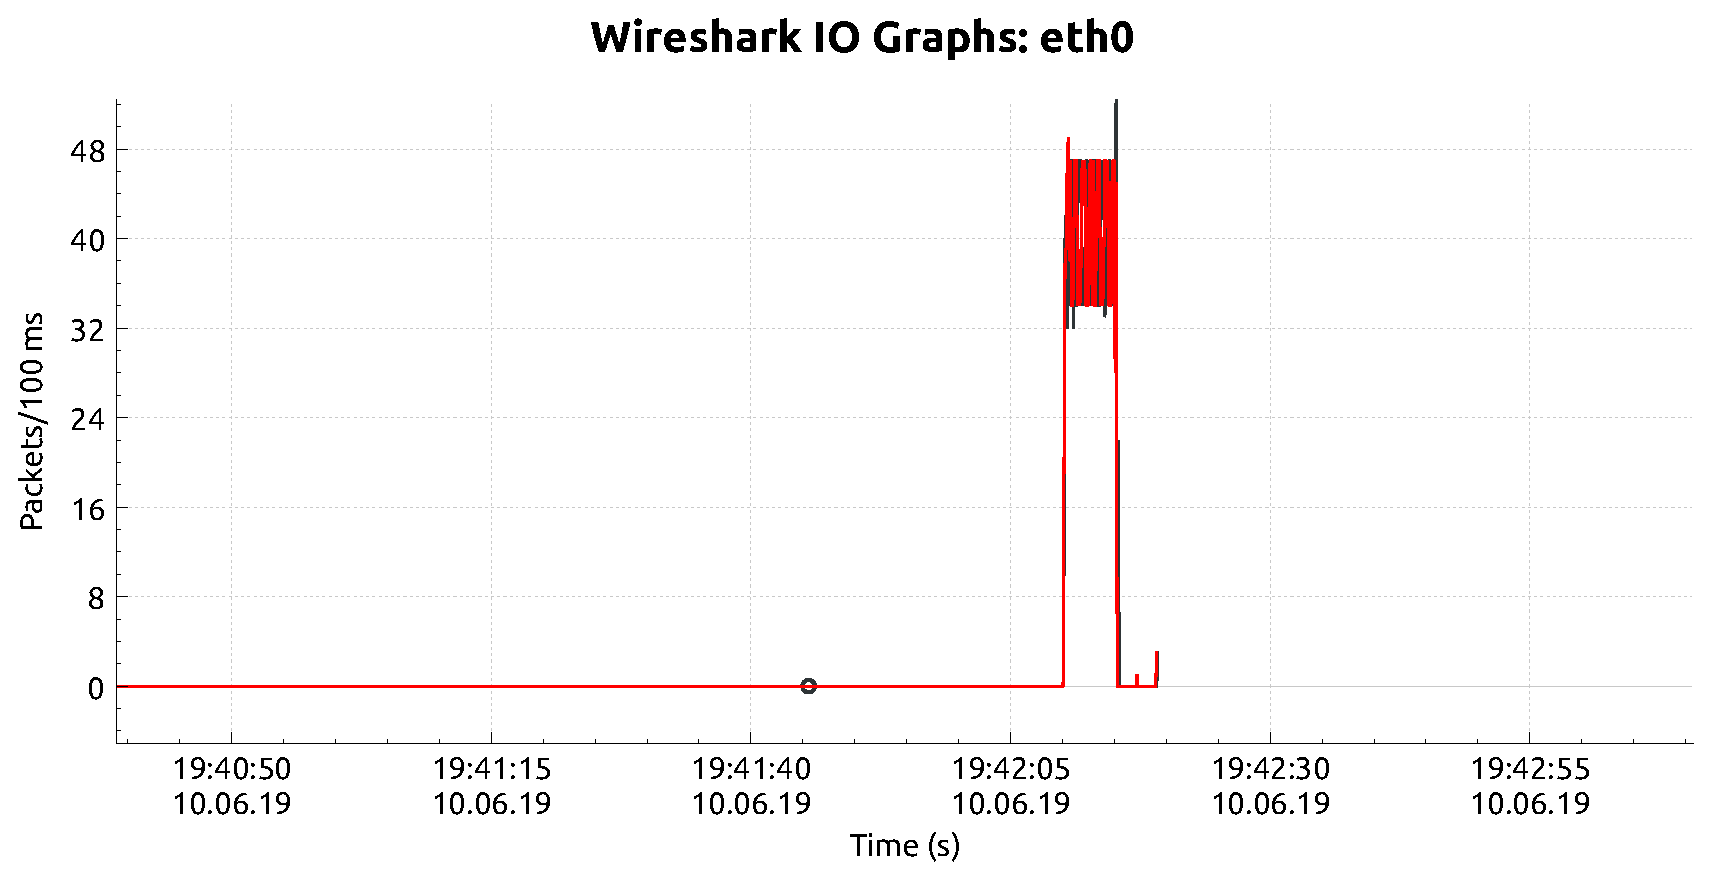
\includegraphics[width=\linewidth]{UDP_H1_test3.pdf}
  		\caption{Velocità F3(nero) e F1(rosso) viste da H1}
	\end{subfigure}	
	\begin{subfigure}[r]{0.5\textwidth}
		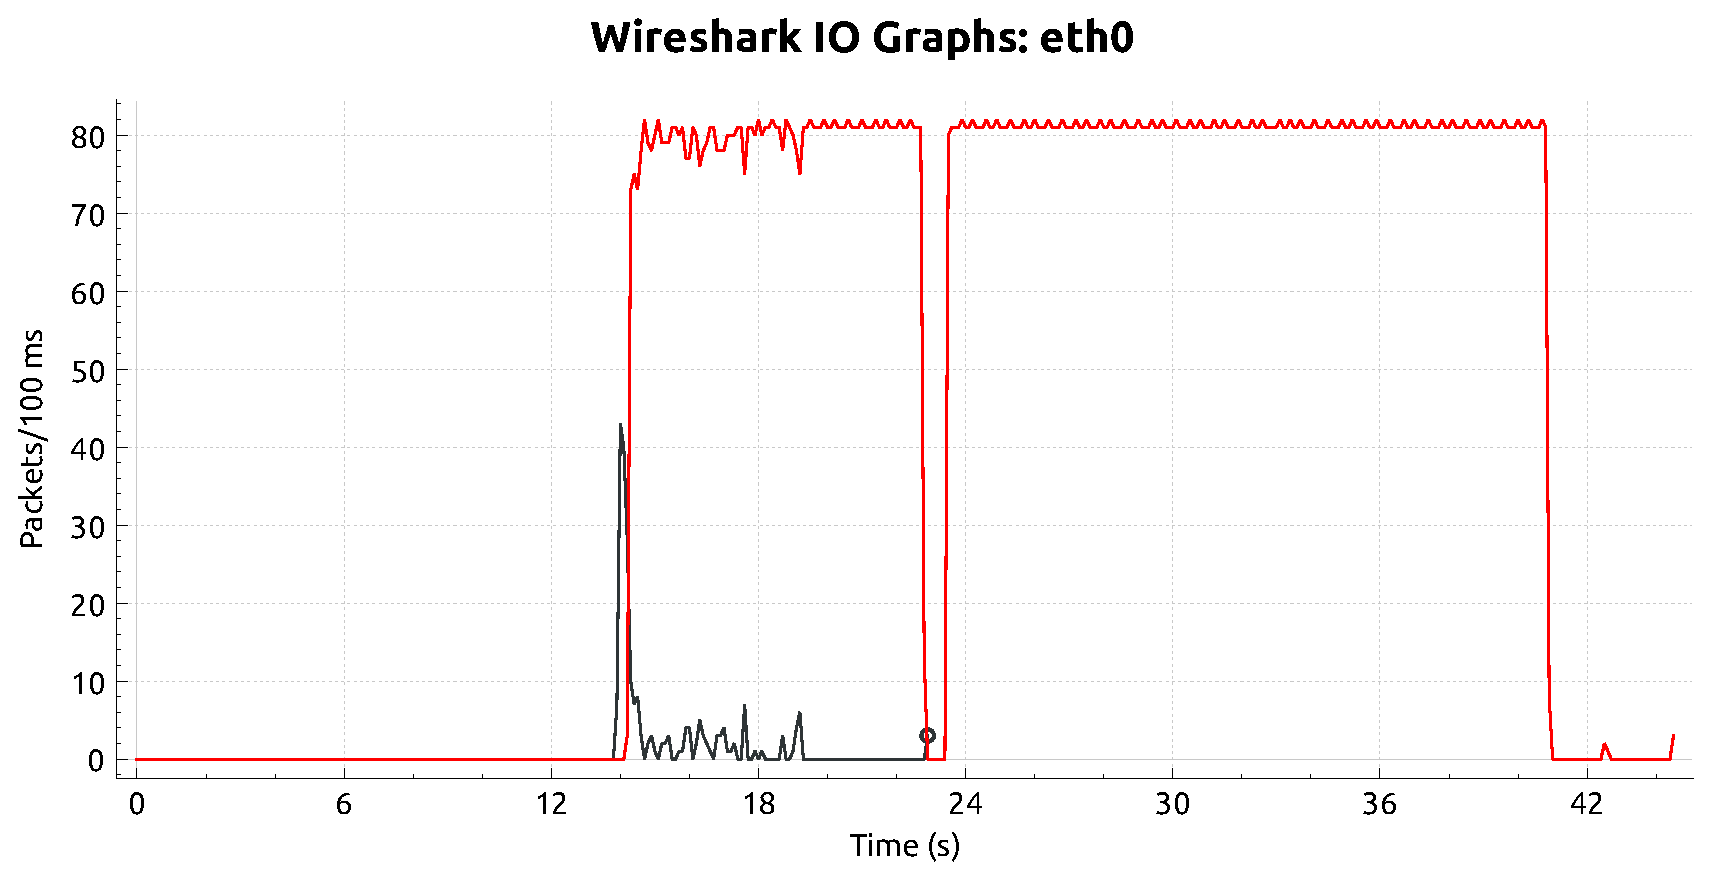
\includegraphics[width=\linewidth]{UDP_H2_test3.pdf}
  		\caption{Velocità F3(nero) e F2(rosso) viste da H2}
	\end{subfigure}}
	\caption{Diagrammi velocità in UDP (test 2)}
\end{figure}

\subsubsection{Test 3}
Per evitare i problemi di connessione incontrati in precedenza abbiamo deciso di eseguire un terzo test avviando prima F3 e F1, e solamente dopo qualche istante F2, in modo da non saturare la banda e permettere tutte le connessioni. Ciò che notiamo dai grafici in \textit{figura 7} e \textit{figura 8} è che F2 monopolizzerà i buffer dello switch finchè non ha terminato la trasmissione, costringendo F1 e F3 a trasmettere molto lentamente.\\
Terminata tale fase F1 e F3 Si dimezzeranno la banda in modo equo, proprio come avveniva già in precedenza nel test 1.\\
Per quanto riguarda la perdita dei pacchetti osserviamo questi risultati su F1 e F3.
\begin{verbatim}
F3
  Bytes  Real s   CPU s Real-MBit/s  CPU-MBit/s   Calls  Real-C/s   CPU-C/s
7360000   12.17    0.02      4.8378   3094.5499    5003    411.06  262942.1
3746240   12.31    0.08      2.4337    379.0686    2546    206.75   32202.6

F1
  Bytes  Real s   CPU s Real-MBit/s  CPU-MBit/s   Calls  Real-C/s   CPU-C/s
7360000   12.23    0.02      4.8149   3031.1454    5003    409.12  257554.7
3756544   12.33    0.11      2.4365    277.5225    2553    206.98   23576.0
\end{verbatim}
Dunque F1 e F3 perderanno entrambi la metà dei pacchetti. Tale risultato è giustificato dai 2 grafici citati in precedenza, infatti in \textit{figura 7} (catturata da H1) possiamo notare come F3 e F1 non "vedano" la congestione sullo switch causata da F2, di conseguenza la quasi totalità dei pacchetti da loro 2 inviati verrà persa. Possiamo trovare un riscontro in \textit{figura 8} (catturata da H2) in cui notiamo che H2 non riceverà alcun pacchetto da parte di H1 finchè F2 non terminerà. Inoltre possiamo notare che questo tempo corrisponde alla metà del tempo impiegato da F1 e F3 per trasferire tutti i pacchetti, possiamo dunque ipotizzare che vi sarà perdita di pacchetti solo del periodo in cui F3 saturerà lo switch e non in quello successivo (il che è coerente con i risultati ottenuti nel primo test).\\
F2 si comporterà in maniera simile se non identica agli altri test, ovvero perderà molti pacchetti
Notare come F3 compirà un picco prima di abbassare la propria velocità e dividere la banda con F1, in quanto appena F2 terminerà F3 riuscirà a riempire l'intero buffer prima che F1 possa intervenire.

\begin{figure}[H]
	\noindent\makebox[\textwidth]{%
	\begin{subfigure}[l]{0.5\textwidth}
		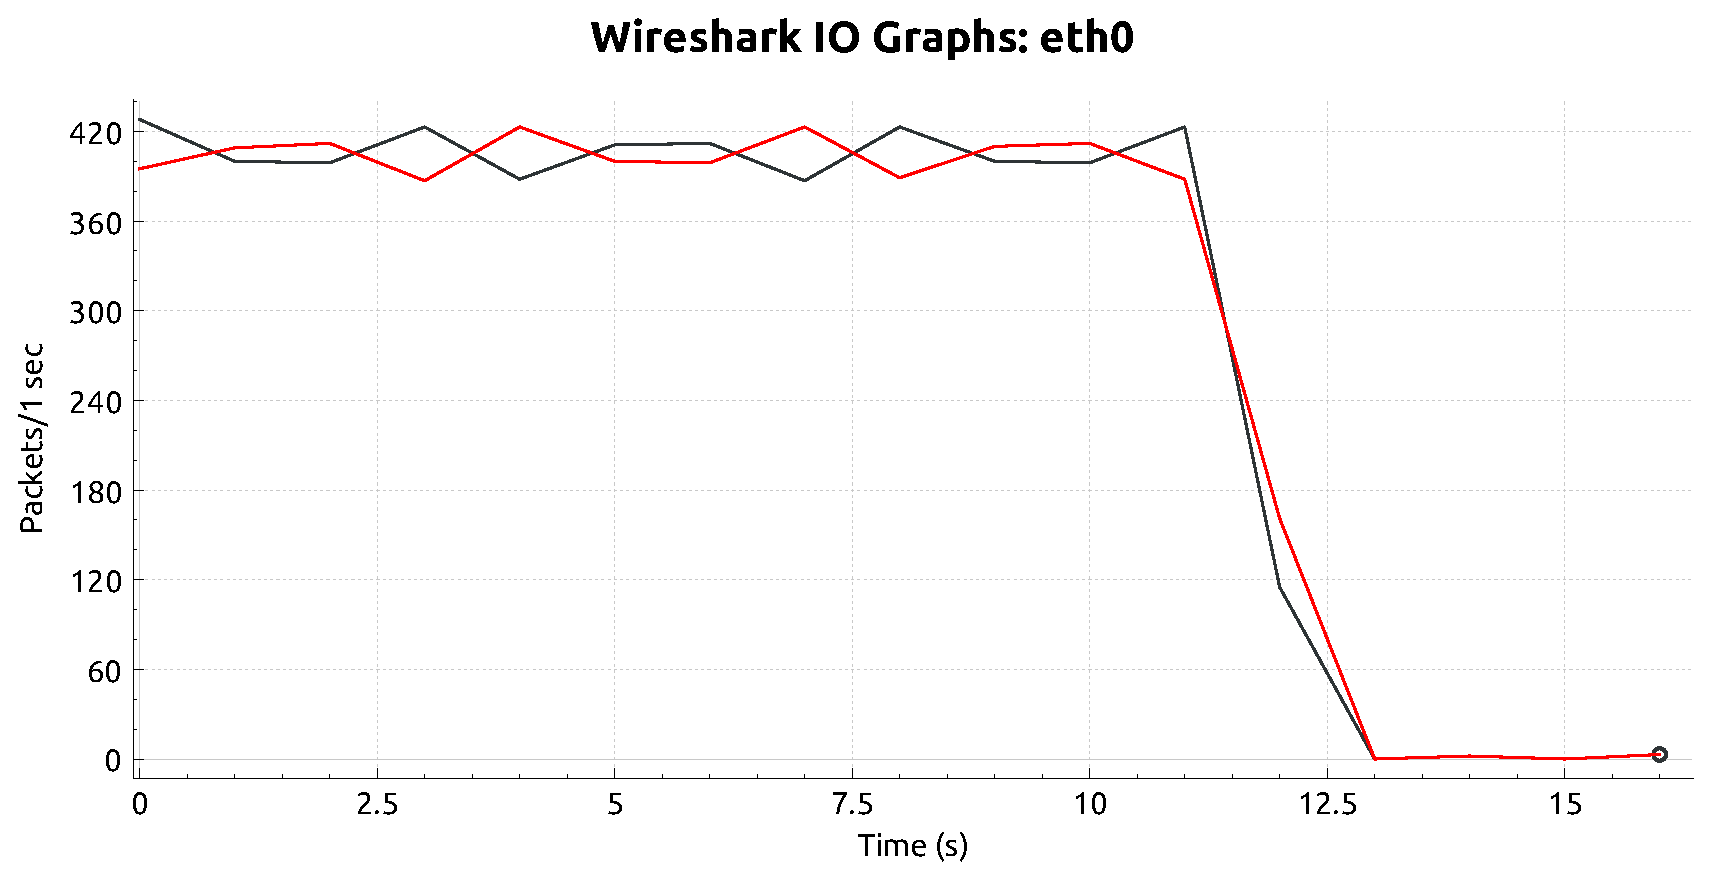
\includegraphics[width=\linewidth]{UDP_H1_test4.pdf}
  		\caption{Velocità F3(nero) e F1(rosso) viste da H1}
	\end{subfigure}	
	\begin{subfigure}[r]{0.62\textwidth}
		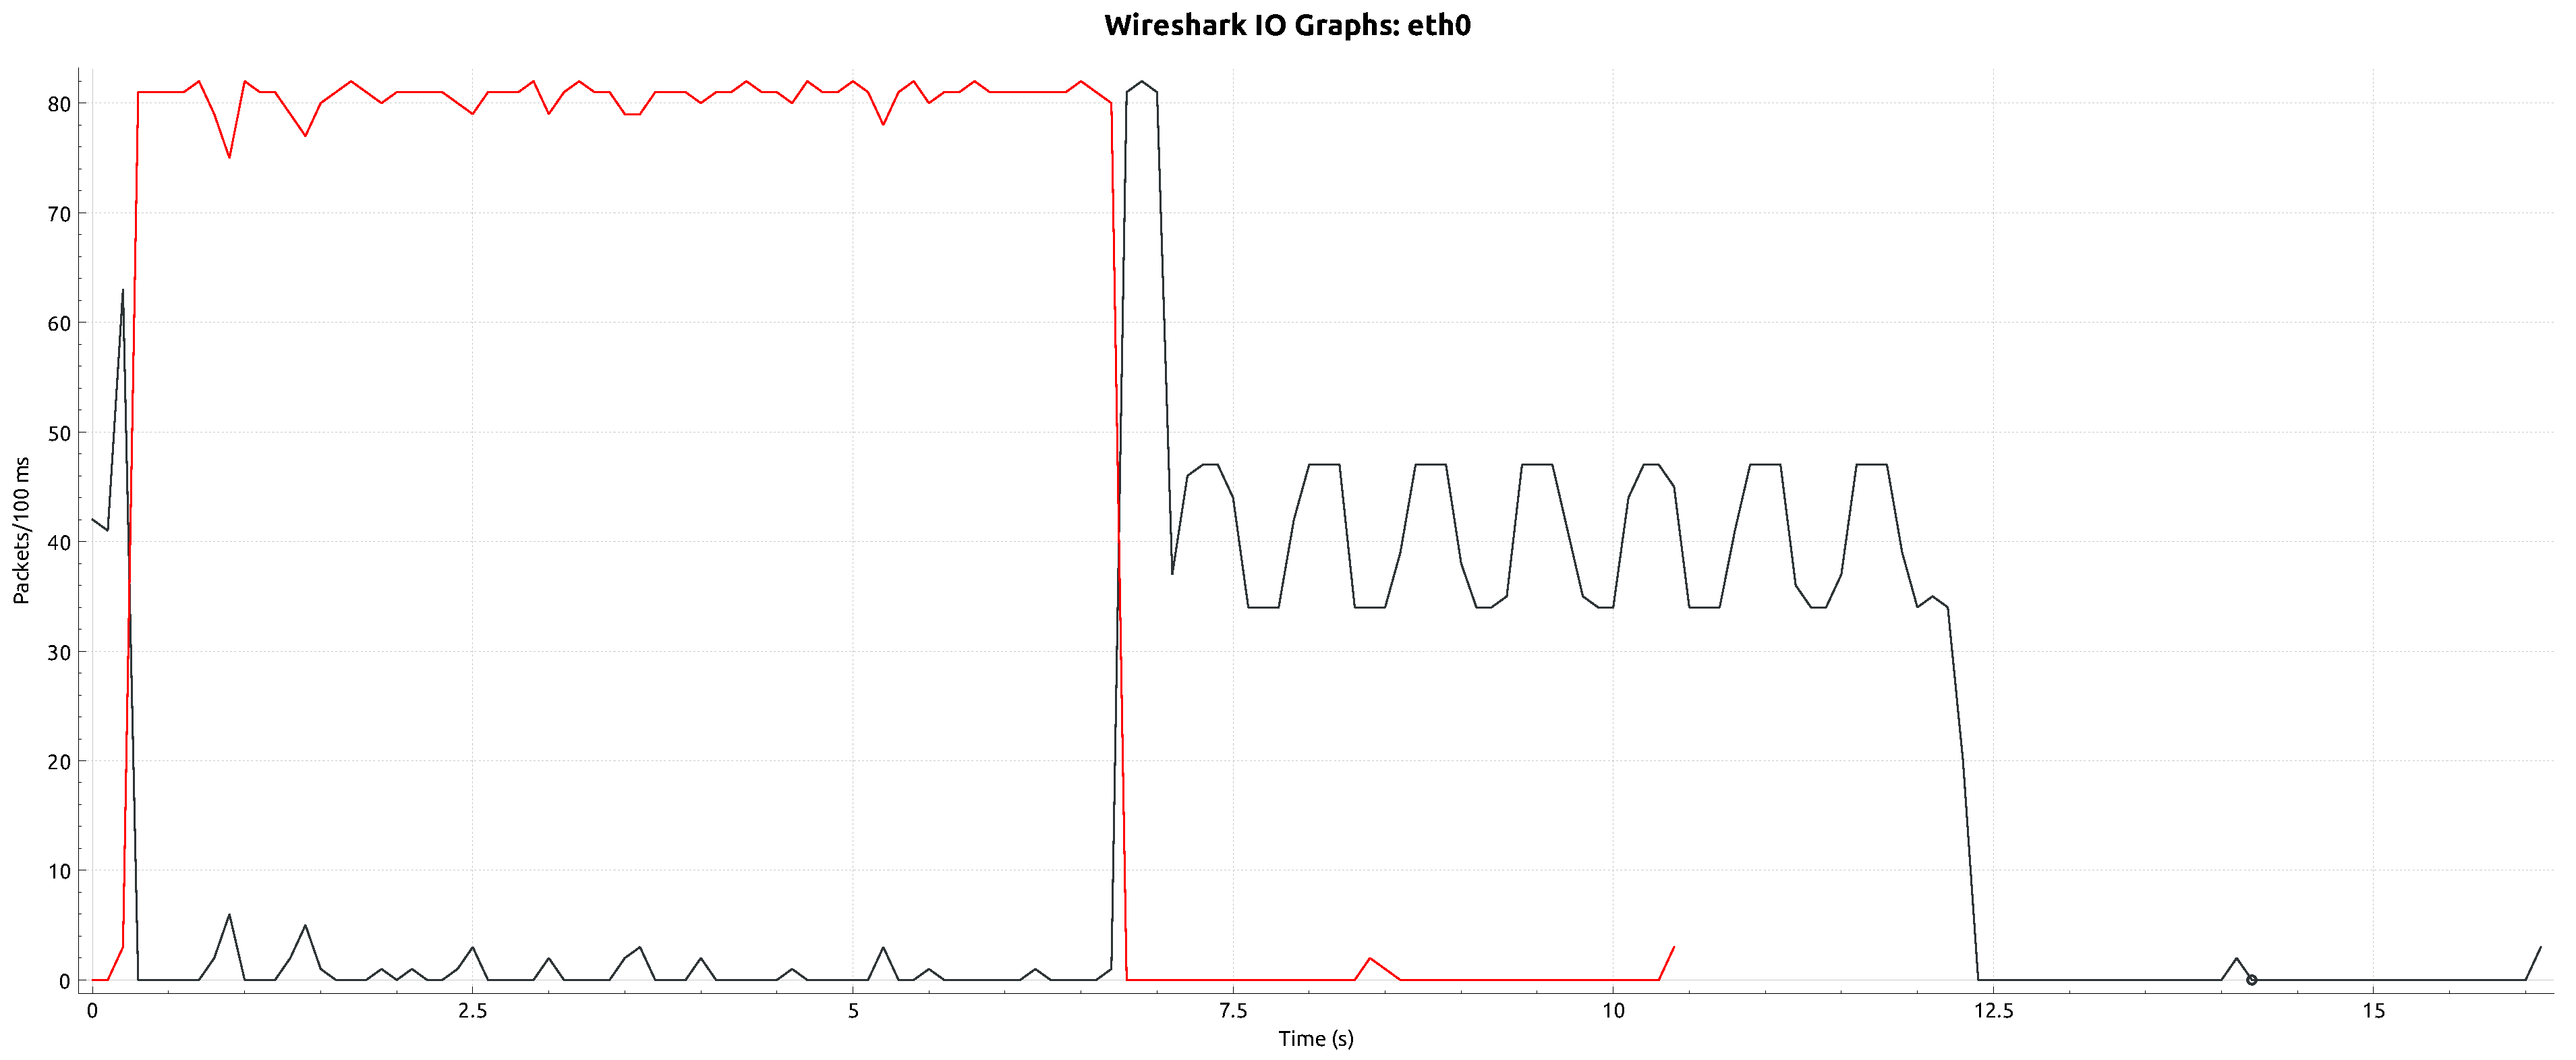
\includegraphics[width=\linewidth]{UDP_H2_test4.pdf}
  		\caption{Velocità F3(nero) e F2(rosso) viste da H2}
	\end{subfigure}}
	\caption{Diagrammi velocità in UDP (test 3)}
\end{figure}

\subsection{Misto}
In questo secondo scenario abbiamo utilizzato nttcp sfruttando sia UDP che TCP, utilizzando i comandi descritti in precedenza.
In particolare F1 è stata settata per comunicare in UDP, mentre le altre 2 in TCP.\\
Come possiamo notare dai grafici in \textit{figura 9} e \textit{figura 10}, F1 ignorerà la congestione dello switch perdendo tuttavia pochi pacchetti e rallentando di conseguenza F3 (poca congestione). Tale perdita è dovuta esclusivamente a F3 che occuperà una piccola parte del buffer in entrata. Possiamo ipotizzare che i buffer dello switch saranno in grado di sostenere al massimo connessioni a 10mb/s prima di raggiungere la saturazione.
\begin{verbatim}
F1
  Bytes  Real s   CPU s Real-MBit/s  CPU-MBit/s   Calls  Real-C/s   CPU-C/s
7360000    6.35    0.02      9.2772   3157.2738    5003    788.28  268271.8
7270208    6.51    0.15      8.9315    394.3511    4940    758.60   33494.5
\end{verbatim}
Infatti F3 essendo TCP sarà in grado di effettuare un controllo sulla congestione e regolare la proprià velocità di conseguenza. Notare inoltre che ciò non andrà a condizionare la velocità di F2, che dovrà solamente condividere una sezione di cavo con F3, la quale causerà pochissima congestione in quanto molto lenta. Infatti possiamo notare in \textit{figura 10} come in seguito alla terminazione di F1 aumenterà la velocità di F3, che si contenderà la banda con F2. Tuttavia F2 sarà sempre più veloce rispetto a F3. Ciò avviene in quanto TCP si troverà a dover creare un'equilibrio in cui non vi sia congestione e vi sia un'equa divisione della banda. Tuttavia partendo da una situazione di disparità tra le due velocità TCP cercherà di instaurare un equilibrio intervenendo il meno possibile sulle connessioni, senza stravolgere l'equilibrio formatosi in precedenza. Si ipotizza che, se la trasmissione di F2 fosse durata di più, con il passare del tempo F3 e F2 sarebbero riusciti a dimezzarsi la banda.
Infine F3 riuscirà ad ottenere l'intera banda.

\begin{figure}[H]
	\noindent\makebox[\textwidth]{%
	\begin{subfigure}[l]{0.61\textwidth}
		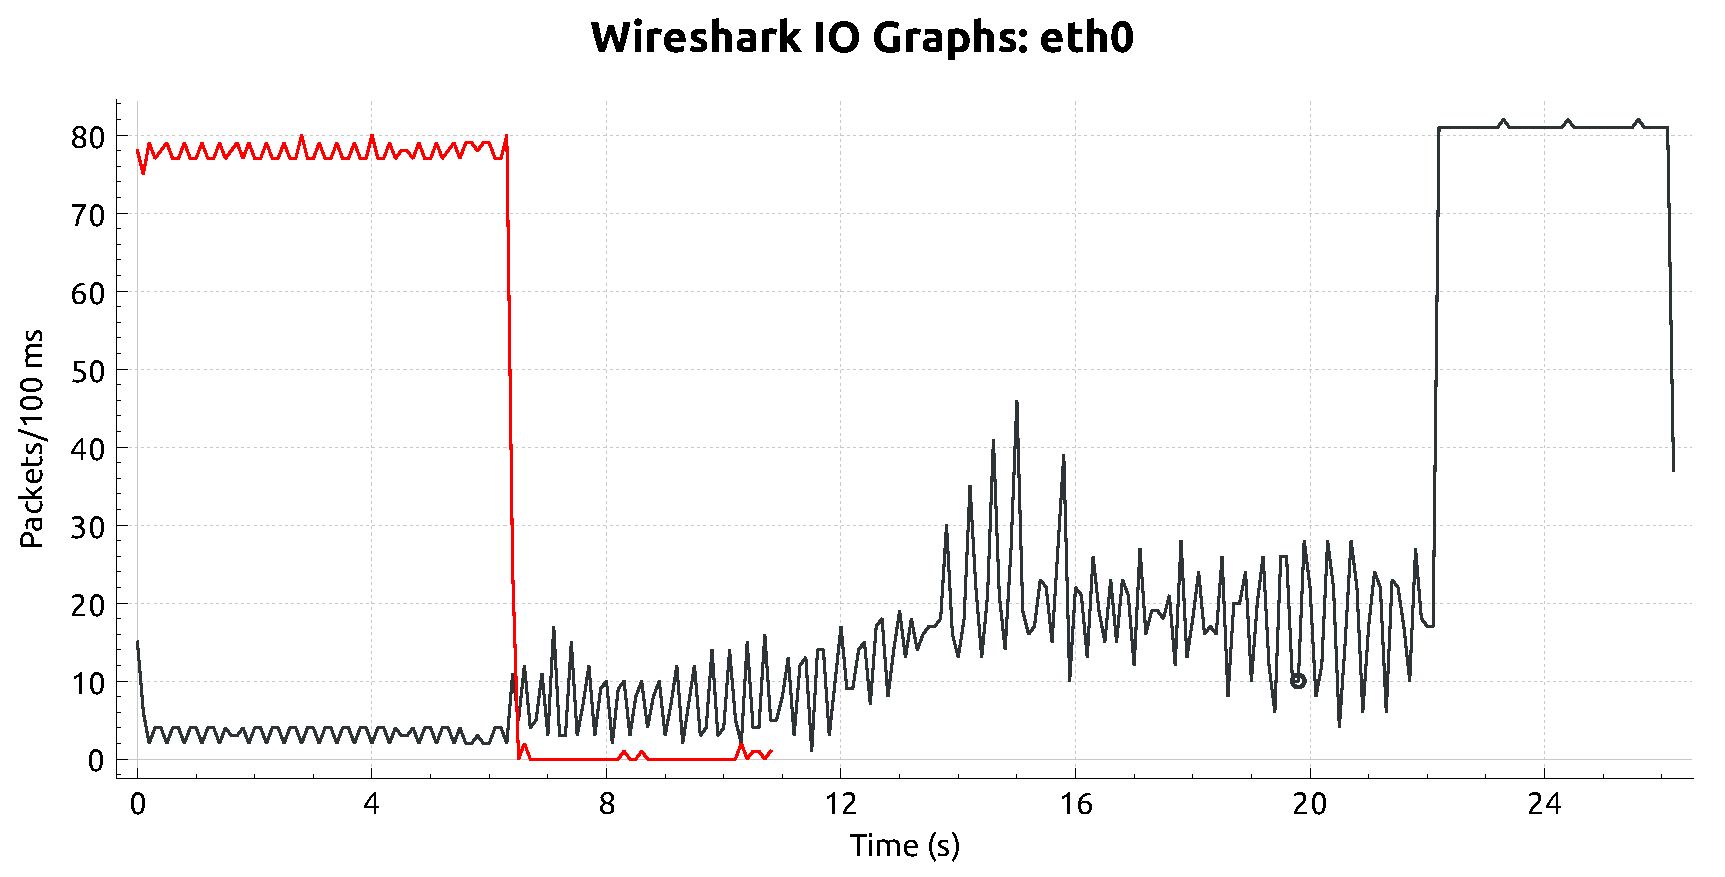
\includegraphics[width=\linewidth]{MIX_H1_test3.pdf}
  		\caption{Velocità F3(nero) e F1(rosso) viste da H1}
	\end{subfigure}	
	\begin{subfigure}[r]{0.5\textwidth}
		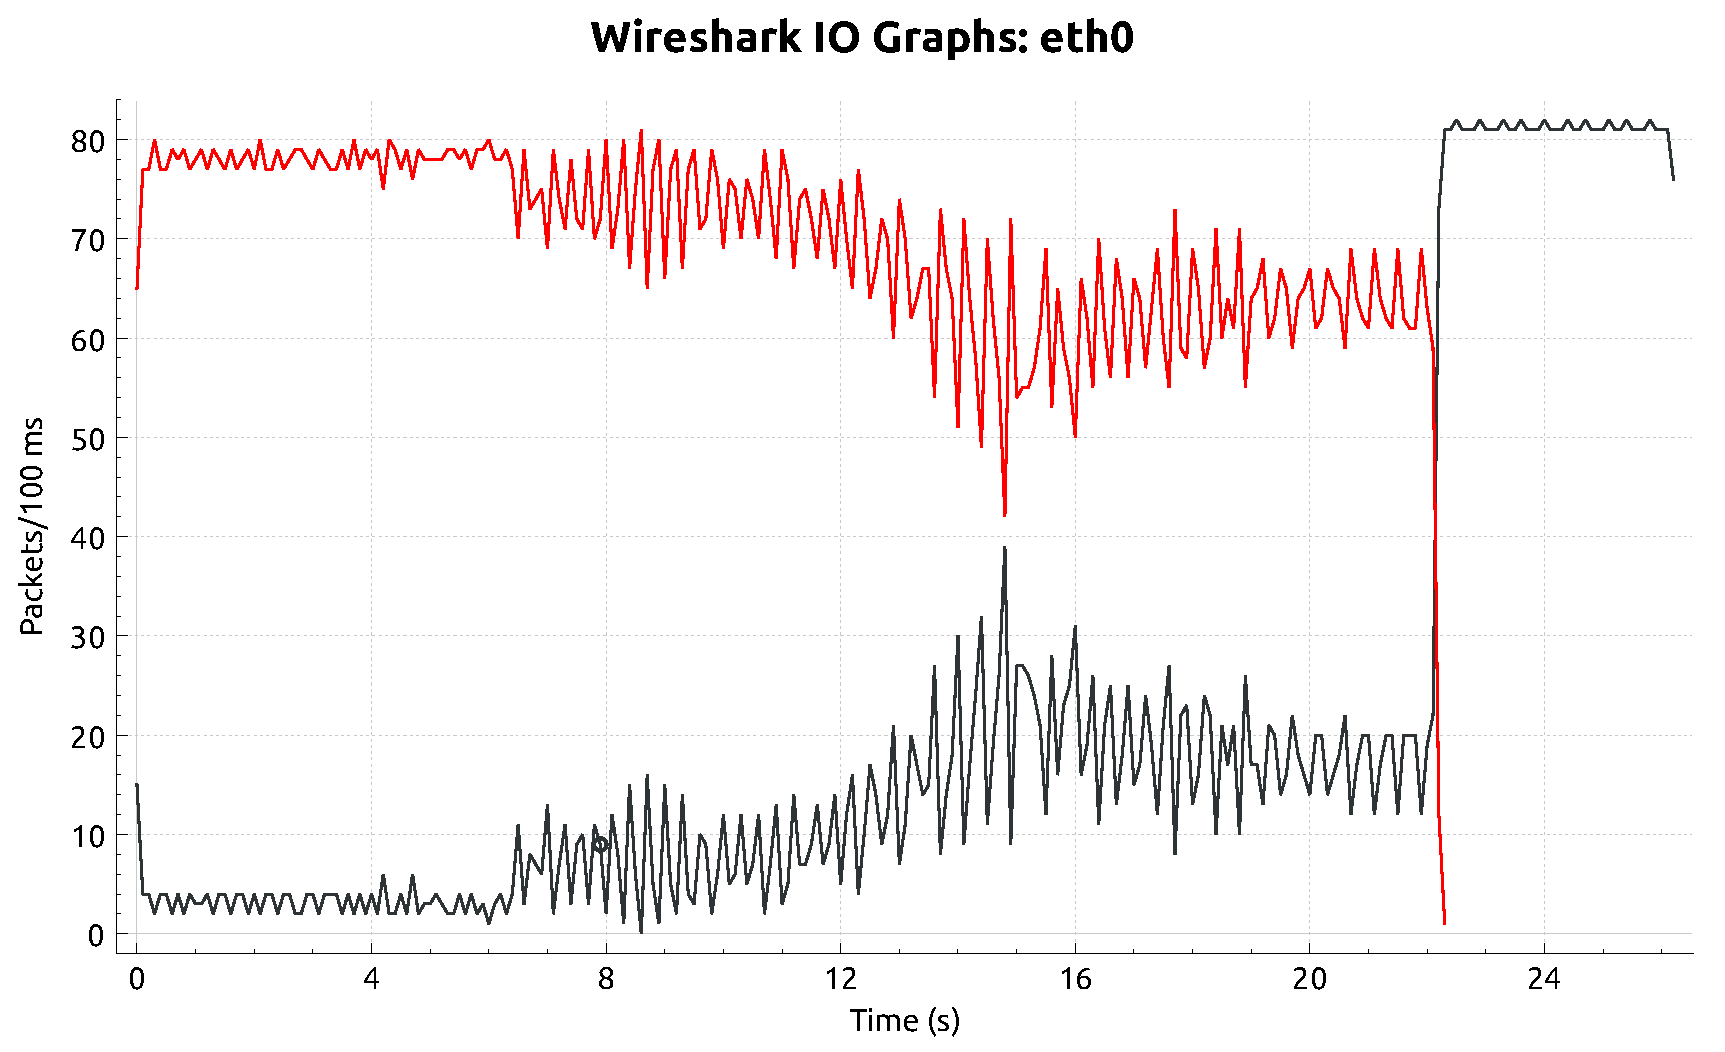
\includegraphics[width=\linewidth]{MIX_H2_test3.pdf}
  		\caption{Velocità F3(nero) e F2(rosso) viste da H2}
	\end{subfigure}}
	\caption{Diagrammi velocità in MISTO}
\end{figure}

\end{document}
